\documentclass[25pt, landscape, blockverticalspace=10mm,  colspace=10mm]{tikzposter}
\tikzposterlatexaffectionproofoff
\geometry{paperwidth=31.1in,paperheight=44in}

\makeatletter
\setlength{\TP@visibletextwidth}{\textwidth-2\TP@innermargin}
\setlength{\TP@visibletextheight}{\textheight-2\TP@innermargin}
\makeatother
% \usepackage{moresize}
\usepackage{graphicx}
% \usepackage[normalem]{ulem}
\usepackage{multirow}
\usepackage{array}
\usepackage{xpatch}
\usepackage[export]{adjustbox}
\usepackage{subfigure}

\usepackage{verbatim}
\usepackage{tikz,times}
\usetikzlibrary{mindmap,backgrounds}
\usetikzlibrary{positioning}
% \pagestyle{empty}

\usepackage{multicol}   
   
\definecolor{darkorange}{rgb}{1.0, 0.35, 0.0}   
\definecolor{darkgreen}{rgb}{0.0, 0.44, 0.0}
\definecolor{columbia}{RGB}{64,104,183}	

\newcommand{\mitem}{{\color{columbia}$\circ$}}
\newcommand{\smitem}{{\color{columbia}--}}

\title{\parbox{\linewidth}{\centering Overview of Commonly-Used Methods to Analyze Exposure to Mixtures in Environmental Epidemiology}} 

\author{Elizabeth A. Gibson$^{{\color{columbia}\dagger}}$, Yanelli Nunez, Marianthi-Anna Kioumourtzoglou}

\institute{
\includegraphics[1.5]{mailman_ehs_4c_horiz.png} \\ \vspace{1ex} {\color{columbia} $^{\dagger}$\url{e.a.gibson@columbia.edu}}}

%\titlegraphic{
\includegraphics[scale=.8]{frame_overview.png}}

\settitle{ \centering \vbox{
{\bfseries \Huge \@title \par}
\vspace*{1em}
{\huge \@author \par} 
\vspace*{1em} 
{\LARGE \@institute}
}}

\usetheme{Default}
\colorlet{blocktitlebgcolor}{columbia}
\colorlet{framecolor}{columbia}

\begin{document}

\maketitle[width = .97\textwidth]

%%%%%%%%%%%%%%%%%%
%% Position QR %%
%%%%%%%%%%%%%%%%%%
\node at(TP@title.south east) [above left = 2] {
\includegraphics[scale = 0.7]{frame_overview.png}};

\begin{columns}

%%%%%%%%%%%%%%%%%%%%%%%%%%%%%%%%%%%%%%%%%%%%%%%%%%%%%%%%%%%%%%%%%%%%%%%%
\column{0.0005}
\column{0.72}

\block{}{\LARGE

\begin{minipage}[t]{0.6\linewidth}
{\color{white}some random text}
\end{minipage}%
\begin{adjustbox}{valign=t}
\begin{minipage}[l]{0.4\linewidth}
\begin{itemize}
     \item[\mitem] Numerous methods exist for environmental mixtures exposure assessment in health studies 
\begin{itemize}
    \item[\smitem] Developed in other fields or for environmental mixtures 
    \item[\smitem] {\bf \color{columbia}Choice of method primarily depends on research question(s)}
\end{itemize}
    \item[\mitem] We present some {\color{columbia}examples} of commonly-used methods
\begin{itemize}
    \item[\smitem] Grouped by research question
    \end{itemize}
\end{itemize}
\end{minipage}
\end{adjustbox}

\vspace{-22ex}

% \centering
    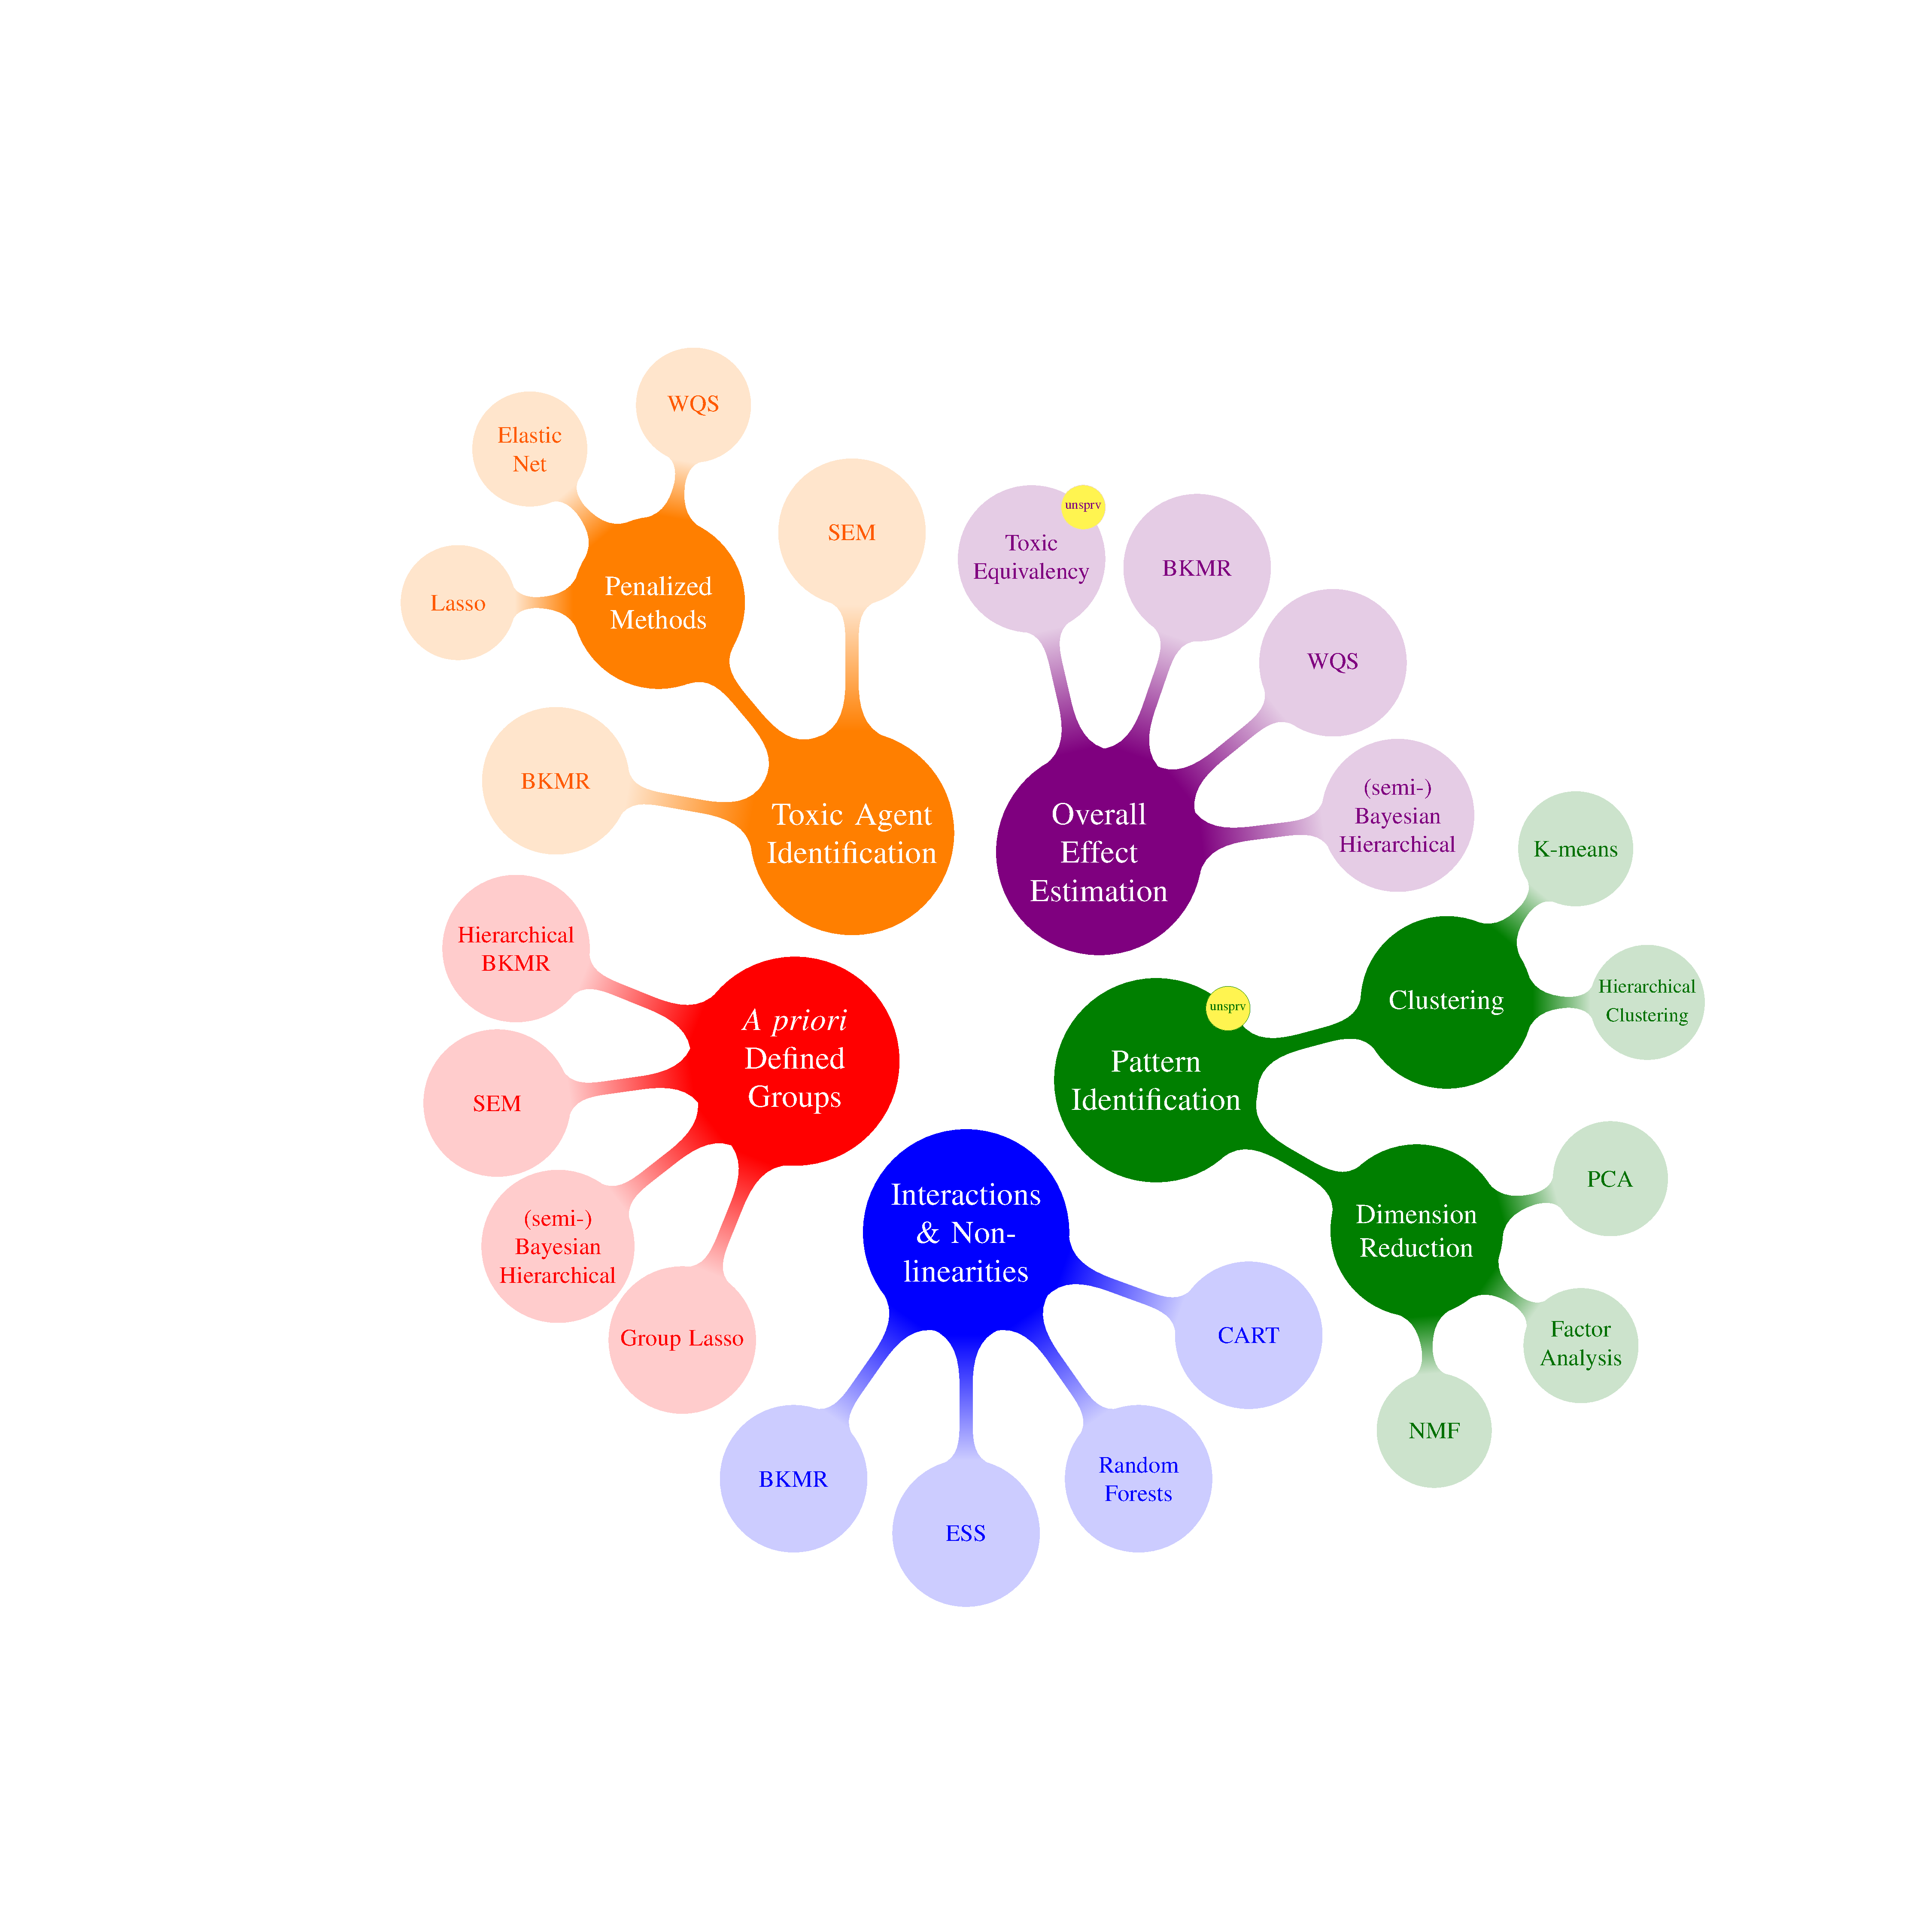
\includegraphics[scale=1.13]{overview.pdf}

\vspace{-6ex}

{\large
\begin{tabular}{cc}  
  \tikz \node [circle, fill = yellow!80, scale=0.5, ultra thin, draw = black] {unsprv};
  & Unsupervised
  \end{tabular}
}

\vspace{-15.7ex}

\begin{flushright}
{\large\color{gray!75}
    \begin{tabular}{ll}
    BKMR    & Bayesian Kernel Machine Regression \\
    CART    & Classification and Regression Trees \\
    ESS     & Exposure Space Smoothing \\
    \multirow{2}{*}{Lasso}   & Least Absolute Shrinkage  \\
            &  and Selection Operator \\
    NFM     & Non-negative Matrix Factorization \\
    PCA     & Principal Component Analysis \\
    SEM     & Structural Equation Modelling \\
    WQS     & Weighted Quantile Sum Regression \\
    \end{tabular}
}    
\end{flushright}
}

%%%%%%%%%%%%%%%%%%%%%%%%%%%%%%%%%%%%%%%%%%%%%%%%%%%%%%%%%%%%%
\column{0.28}


\block{Other Considerations for \\ Method Selection}{\LARGE
\begin{enumerate}
\item No single method outperforms all others for {\color{columbia}all} potential questions
\item {\color{columbia} Interpretability}
\item {\color{columbia} Robustness} 
\item Computational scalability 
\begin{itemize}
    \item[\smitem] As dimensionality increases ($N$ or $p$) some methods may fail 
\end{itemize}
\item Exploration vs. hypothesis testing
\item Not a good idea to ``blindly'' use methods from other fields 
\begin{itemize}
    \item[\smitem] They were developed for different \\ purposes!
    \item[\smitem] May need to adjust them first
\end{itemize}
\end{enumerate}
}

\block{To supervise or not?}{\LARGE
    \begin{enumerate}
        \item Do we want to inform policy?
        \begin{itemize}
            \item[{\color{columbia}$\rightarrow$}] Identify common exposure {\color{columbia} patterns}, independent of outcomes, on which we can act 
            \begin{itemize}
            \item[\smitem] Through regulatory action, targeted interventions etc
            \end{itemize}
        \end{itemize}
        \item Or better understand certain biological pathways?
        \begin{itemize}
            \item[{\color{columbia}$\rightarrow$}] Must include the outcome of interest
        \end{itemize}
    \end{enumerate}
}

\block{}{
\centering\Large Support by NIEHS PRIME R01 ES028805,\\ F31 ES030263 and P30 ES009089}

\column{0.0005}
\end{columns}
\end{document}

% \block{}{
% \begin{tikzfigure}
% \vspace{-1ex}
% 
\includegraphics[scale = 0.95]{mailman_ehs_4c_horiz.png}
% \vspace{-0.5ex}
% \end{tikzfigure}
% }